\question Jaime estudia Medicina. En una clase ha aprendido que hay una nueva generación de fármacos en los que la cantidad de
sustancia activa decae poco a poco hasta que el cuerpo la elimina completamente. Por ejemplo, un enfermo toma una
medicina con 8 mg de sustancia activa, la cual decae 0.5 mg cada dos días. Por lo que su profesor les solicita que describan
la relación entre cantidad de sustancia activa y los días que dura dentro del cuerpo.

\begin{parts}
    \setlength{\columnsep}{30pt}
    \begin{multicols}{2}
        \part[5] Completa la Tabla \ref{tab:farmacos} en la que se calcula diariamente la cantidad de sustancia activa dentro del enfermo.\\[0.1cm]

        \begin{figure}[H]
            \centering
            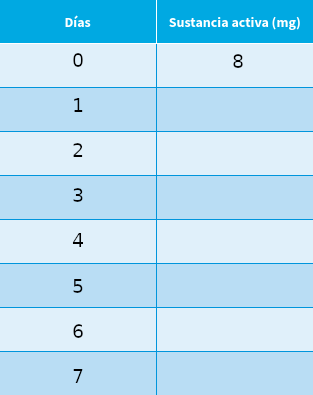
\includegraphics[width=0.6\linewidth]{../images/farmacos}
            \captionof{table}{Tabla que relaciona la cantidad de sustancia activa de acuerdo con los d\'ias.}
            \label{tab:farmacos}
        \end{figure}

        \part[5] Traza la gráfica en la Figura \ref{fig:farmacos_tabla} que describe la relación de la sustancia activa con los días que pasan. ¿La gráfica es ascendente o descendente?

        \begin{figure}[H]
            \centering
            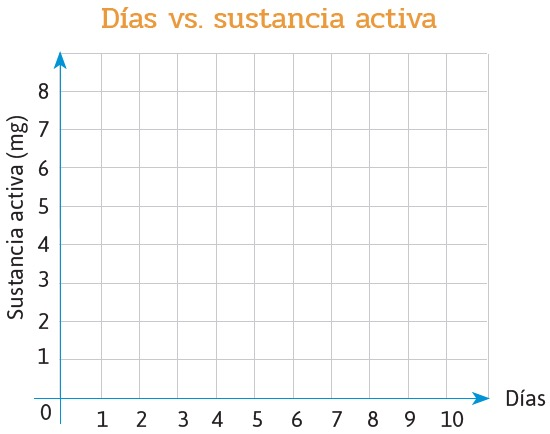
\includegraphics[width=0.9\linewidth]{../images/farmacos_tabla}
            \captionof{figure}{Gráfica que relaciona la cantidad de sustancia activa de acuerdo con los d\'ias.}
            \label{fig:farmacos_tabla}
        \end{figure}

    \end{multicols}

    % \part ¿Cómo cambia la cantidad de sustancia activa conforme pasan los días? ¿Puedes identificar un patrón en la disminución de la sustancia activa? ¿Cuál es?
    % \part ¿Cómo se relaciona ese patrón con la constante de proporcionalidad?
    \part[2] ¿Cuál es la razón de cambio? ¿Cómo se relaciona ésta con la constante de proporcionalidad? ¿Cuál es? Explica su obtención.

    \begin{solutionbox}{2cm}

    \end{solutionbox}

    \part[2] Escribe una expresión algebraica que describa la situación. ¿Cuál es el valor de la pendiente y de la ordenada al origen? Describe su obtención:

    \begin{solutionbox}{2cm}

    \end{solutionbox}

    \part[2] ¿En cuántos días la sustancia activa queda totalmente eliminada del organismo del enfermo? Explica.

    \begin{solutionbox}{2cm}

    \end{solutionbox}

    \newpage

    {
        \printanswers
        \part[2] ¿Cómo es el tiempo que permanece en el cuerpo de un paciente, una sustancia activa
        de 8 mg que decae 0.5 mg cada día con relación al tiempo que permanece la sustancia activa al inicio de este problema?

        \begin{oneparchoices}
            \CorrectChoice Es la mitad
            \choice Es el mismo
            \choice Es el doble
            \choice No hay relación
        \end{oneparchoices}

        \part[2] ¿Cómo es el tiempo que permanece en el cuerpo de un paciente, una sustancia activa de 4 mg que decae
        0.5 mg cada 2 días con relación al tiempo que permanece la sustancia activa al inicio de este problema?

        \begin{oneparchoices}
            \choice Es la mitad
            \CorrectChoice Es el mismo
            \choice Es el doble
            \choice No hay relación
        \end{oneparchoices}
    }
    \part[2] ¿Cómo es el tiempo que permanece en el cuerpo de un paciente, una sustancia activa de 8 mg que decae 1 mg
    por día con relación al tiempo que permanece la sustancia activa del inciso anterior?

    \begin{oneparchoices}
        \choice Es la mitad
        \choice Es el mismo
        \CorrectChoice Es el doble
        \choice No hay relación
    \end{oneparchoices}

    \part[2] ¿Cómo es la razón de cambio de una sustancia activa de 8 mg en el cuerpo humano que decae 0.5 mg cada medio día con
    relación a la razón de cambio de la sustancia del inciso anterior?

    \begin{oneparchoices}
        \CorrectChoice Es igual
        \choice Es mayor
        \choice Es menor
        \choice No hay relación
    \end{oneparchoices}

    \part[2] ¿Cómo es la razón de cambio de una sustancia activa de 8 mg en el cuerpo humano que decae 1 mg cada dos días
    días con relación a la razón de cambio de la sustancia del inciso anterior?

    \begin{oneparchoices}
        \choice Es la mitad
        \CorrectChoice Es el mismo
        \choice Es el doble
        \choice No hay relación
    \end{oneparchoices}

    \part[5] Ordena las sustancias de mayor (5) a menor (1) según el tiempo que permanecen en el cuerpo humano.

    \begin{choices}
        \choice \fillin[200][0.5cm] Sustancia de 8 mg que decae 0.5 mg cada medio día.
        % \choice \fillin[200][0.5cm] Sustancia de 8 mg que decae 0.5 mg diario.
        \choice \fillin[200][0.5cm] Sustancia de 4 mg que decae 1 mg cada dos días.
        \choice \fillin[200][0.5cm] Sustancia de 10 mg que decae 1 mg diario.
        \choice \fillin[200][0.5cm] Sustancia de 6 mg que decae 0.5 mg diario.
    \end{choices}

\end{parts}

